\chapter{Естественно-языковые интерфейсы ostis-систем}
\chapauthortoc{Никифоров С.~А.\\Гойло А.~А.\\Цянь Л.}
\label{chapter_nl_interfaces}

\vspace{-7\baselineskip}

\section*{Введение в Главу~\ref{chapter_nl_interfaces}}

В настоящее время существует большое количество различных \textit{интерфейсов} компьютерных систем, что усложняет интероперабельность между такими системами и людьми в силу необходимости ознакомления с интерфейсом каждой новой системы, который зачастую может быть не интуитивно понятен.

Одной из основных особенностей \textit{ostis-систем} должен являться \textit{пользовательский интерфейс}, способный обеспечить эффективное взаимодействие пользователя с системой в условиях его общей профессиональной неподготовленности.

Одной из наиболее естественных и удобных форм передачи информации между людьми является речь, что обуславливает все большее распространение \textit{естественно-языковых интерфейсов} (см.~\scncite{GlobalMarket}).
В настоящий момент времени уже ни у кого не вызывает сомнения, что данная форма взаимодействия человека и машины играет и будет играть значительную роль во взаимодействии с различными компьютерными системами.

Однако необходимо отметить, что большое многообразие \textit{языков} (как \textit{естественных}, так и \textit{искусственных}) ведет к необходимости упрощения процесса создания таких \textit{интерфейсов} для каждого отдельно взятого \textit{языка}.

Разработка естественно-языковых интерфейсов для современных интеллектуальных систем, основанных на знаниях, в общем случае требует учета следующих двух основных аспектов:
\begin{textitemize}
	\item особенности обрабатываемого естественного языка;
	\item диапазон базы знаний интеллектуальных систем, то есть широта знаний в базах знаний интеллектуальных систем.
\end{textitemize}

На данный момент существует большое количество методов обработки естественного языка, которые в основном можно разделить на два направления:
\begin{textitemize}
	\item методы на основе правил и лингвистических знаний;
	\item методы машинного обучения, основанные на математической статистике и теории информации.
\end{textitemize}

В основе большинства подходов к обработке и пониманию \textit{естественного языка} лежит машинное обучение (см.~\scncite{Pais2022},~\scncite{Trajanov2022}).
Несомненно, для большинства широко распространенных \textit{языков} модели для обработки естественного языка работают очень хорошо и совершенствуются с каждым днем, но несмотря на успехи в данной области, данный подход имеет ряд недостатков:
\begin{textitemize}
    \item проблемы при работе с различными областями, например, значения слов или предложений могут быть различными в зависимости от \textit{предметной области}.
    Таким образом, модели для NLP могут хорошо работать для отдельной \textit{предметной области}, но не подходить для широкого применения (см.~\scncite{Khurana2022});
    \item создание новой модели модели требует наличия большого объема данных, а качество таких данных напрямую влияет на качество получаемой модели, что ведет к большим затратам на ее обучение (см.~\scncite{Strubell2019}, \scncite{LLM});
    \item данные модели представляют собой "черный ящик"{}, так как данные модели не обладают средствами для обоснования своего вывода;
    \item каждая такая модель решает только свой узкий класс задач, отсутствует общий подход к обработке естественного языка (см.~\scncite{Khurana2022}).
\end{textitemize}

Данные недостатки используемых методов являются причиной части недостатков современных систем, реализующих \textit{естественно-языковой интерфейс}, так, несмотря на то, что сейчас существует большое количество речевых ассистентов, создаваемых разными компаниями (см.~\scncite{Alexa}, \scncite{Siri},\scncite{GoogleAssistant}, \scncite{Cortana}).
Они обладают схожими недостатками, например, исключительно распределенной реализацией, в силу недостаточной для запуска ресурсоемких моделей производительности устройств конечных пользователей.
Это в свою очередь ведет к проблемам с приватностью (см.~\scncite{Hoy2018}).

Подмодуль понимания речи данных систем формирует конструкцию, отражающую смысл сообщения используя \textit{фреймовую модель}.
Упрощенный пример такой конструкции приведен на~\textit{\nameref{fig:message_intents}}.

\begin{figure}[H]
    \caption{Рисунок. Иллюстрация формализованного смысла сообщения}
    \centerline{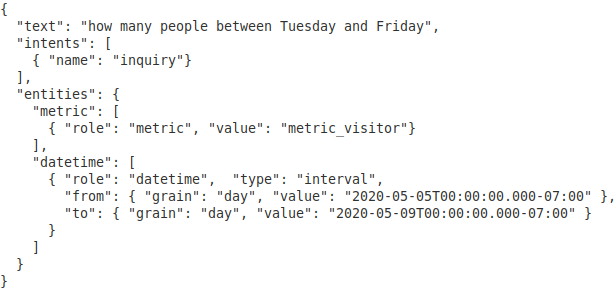
\includegraphics[scale=0.55]{images/part4/chapter_nl_interfaces/message_intents}}
    \label{fig:message_intents}
\end{figure}

При этом для представления результатов промежуточных этапов обработки используются иные форматы, модули которые их реализуют не имеют какой-либо единой основы и взаимодействуют посредством специализированных \textit{программных интерфейсов} между ними, что приводит к несовместимости способов представления результатов на различных этапах обработки и конечного результата обработки текстов.
Данная несовместимость в свою очередь ведет к существенным накладным расходам при разработке такой системы и в особенности при ее модификации.

В качестве решения проблемы совместимости предлагается использование подхода к обработке \textit{естественного языка} на основе его \textit{формальной модели} в виде набора \textit{онтологий}, сформированных с использованием универсальных средств представления знаний, что будет способствовать интероперабельности как компонента по обработке \textit{естественного языка} в целом с другими компонентами системы, так и между составляющими самого данного компонента.

Целью главы является формирование модели \textit{интерфейса}, в основе которой лежит подход к обработке \textit{естественного языка} на основе \textit{онтологий}, содержащих формальное описание \textit{естественного языка}.

\textit{естественно-языковой интерфейс} --- \textit{SILK-интерфейс} (Speech --- речь, Image --- образ, Language --- язык, Knowledge --- знание), обмен информацией между компьютерной системой и пользователем в котором происходит за счет диалога.

\textbf{\textit{речевой интерфейс}} --- \textit{SILK-интерфейс}, обмен информацией в котором происходит за счет диалога, в процессе которого компьютерная система и пользователь общаются с помощью речи.
Данный вид интерфейса наиболее приближен к естественному общению между людьми.

В предлагаемом подходе можно выделить следующие этапы обработки \textit{естественного языка}:
\begin{textitemize}
    \item лексический анализ;
    \item синтаксический анализ;
    \item понимание сообщения.
\end{textitemize}

В свою очередь, лексический анализ в включает в себя \textit{декомпозицию} текста на токены и их сопоставление с \textit{лексемами}.

Понимание сообщения сводится к генерации вариантов значения сообщения и выбору из них корректного на основании \textit{контекста}, а также погружение его в данный \textit{контекст}.

Ниже приведена структура \textit{решателя задач} \textit{естественно-языкового интерфейса}.

\begin{SCn}

    \scnheader{Решатель задач естественно-языкового интерфейса}
    \begin{scnrelfromset}{декомпозиция абстрактного sc-агента}
        \scnitem{Абстрактный sc-агент лексического анализа}
        \begin{scnindent}
            \begin{scnrelfromset}{декомпозиция абстрактного sc-агента}
                \scnitem{Абстрактный sc-агент декомпозиции текста на токены}
                \scnitem{Абстрактный sc-агент сопоставления токенов с лексемами}
            \end{scnrelfromset}
        \end{scnindent}
        \scnitem{Абстрактный sc-агент синтаксического анализа}
        \scnitem{Абстрактный sc-агент понимания сообщения}
    \end{scnrelfromset}

\end{SCn}

В свою очередь, \textit{Абстрактный sc-агент понимания сообщения} декомпозируется на:

\begin{SCn}

    \scnheader{Агент понимания сообщения}
    \begin{scnrelfromset}{декомпозиция абстрактного sc-агента}
        \scnitem{Абстрактный sc-агент генерации вариантов значения сообщения}
        \scnitem{Абстрактный sc-агент выбора и обновления контекста}
        \begin{scnindent}
            \begin{scnrelfromset}{декомпозиция абстрактного sc-агента}
                \scnitem{Абстрактный sc-агент разрешения контекста}
                \scnitem{Абстрактный sc-агент выбора смысла сообщения на основе контекста}
                \scnitem{Абстрактный sc-агент погружения сообщения в контекст}
            \end{scnrelfromset}
        \end{scnindent}
    \end{scnrelfromset}

\end{SCn}

\section{Синтаксический анализ естественно-языковых сообщений, входящих в ostis-систему}
\label{section_natural_language_messages_syntax_analysis}

В данной главе мы не будем подробно описывать процесс лексического анализа и его ключевые аспекты (такие как, например, устранение омонимии) --- данный вопрос требует дополнительной проработки.
Вместо этого, акцент будет сделан на этапе синтаксического анализа, предварительным условием которого является уже проведенный лексический анализ текста \textit{естественного языка}.

\begin{SCn}

    \scnheader{действие. лексический анализ естественно-языкового сообщения}
    \begin{scnrelfromset}{обобщенная декомпозиция}
        \scnitem{действие. декомпозиция текста на токены}
        \scnitem{действие. сопоставление токенов с лексемами}
    \end{scnrelfromset}

\end{SCn}

Лексический анализ представляет собой декомпозицию текста на последовательность токенов и сопоставление \textit{лексем} с получившимися при данной декомпозиции токенами.
Следует отметить, что данные токены при необходимости могут сопоставляться не с \textit{лексемами}, а с их подмножествами, входящими в ее \textit{морфологическую парадигму}, соответствующими определенным грамматическим категориям: падежу, числу, роду и так далее.

Результат лексического анализа представлен на~\textit{\nameref{fig:lexical_result}}.

\begin{figure}[H]
    \caption{SCg-текст. Иллюстрация результата лексического анализа.}
    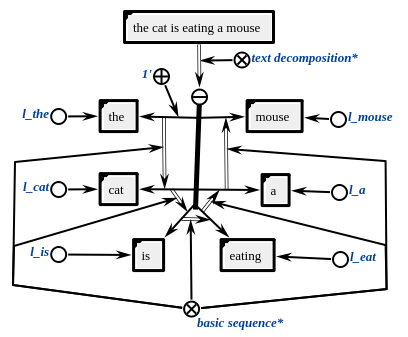
\includegraphics[scale=0.8]{images/part4/chapter_nl_interfaces/lexical}
    \label{fig:lexical_result}
\end{figure}

Для осуществления лексического анализа, в базе знаний системы также должен присутствовать словарь, содержащий \textit{лексемы} и их различные формы.

Под \textit{лексемой} понимается единица словарного состава языка, которая представляет собой множество всех форм некоторого слова.


В данной главе мы также рассмотрим, как могут учитываться особенности конкретных естественных языков при разработке естественно-языковых интерфейсов ostis-систем на примере китайского языка.

Традиционно в лингвистике структура слова изучается в рамках морфологии.
Носителем морфологической парадигмы и ключевым элементом анализа является лексема.
Однако, в китайском языке из-за письменной традиции (текст китайского языка состоит из последовательности иероглифов без пробелов), наименьшей единицей при обработке текстов считается единица сегментации.
Описание единицы сегмантации приводится в государственном стандарте «Стандарт сегментации слов современного китайского языка, используемый для обработки информации».

\begin{comment}
	

\begin{SCn}
	\scnheader{единица сегментации}
	\scnidtfdef{базовая единица для обработки китайского языка, имеющая определенные семантические или грамматические свойства}
	\scnsubset{файл}
\end{SCn}

Стоит отметить, что термин единица сегментации используется при компьютерной обработке текстов китайского языка и не полностью совпадает с описанием слов в китайской лингвистике.

Кроме того, в китайском языке отсутствуют четкие показатели категорий числа, падежа и рода, в отличие от русского языка и других европейских языков.
Функцию слова в китайском языке можно определить не на основании морфемного состава, а при помощи анализа связей этого слова с другими словами.
В связи с этим, в процессе анализа текстов китайского языка сначала необходимо выполнить лексический анализ, разбивающий поток иероглифов в тексте китайского языка на отдельные значимые единицы сегментации.

Результат декомпозиции предложения на единицы сегментации представлен на~\textit{\nameref{fig:segment-chinese}}.

\begin{figure}[H]
	\caption{SCg-текст. Иллюстрация результата лексического анализа предложения на китайском языке}
	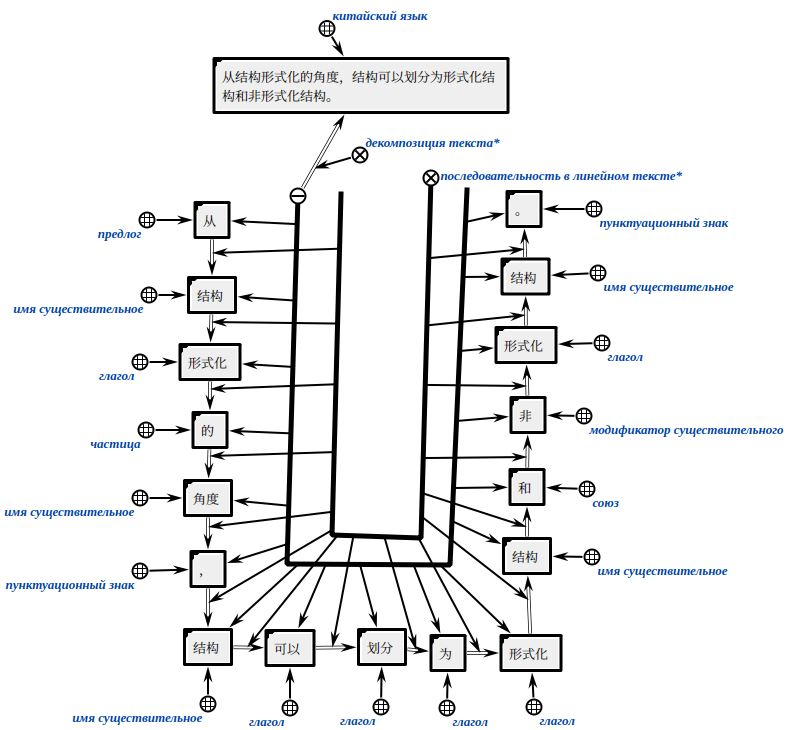
\includegraphics[scale=0.6]{images/part4/chapter_chinese/segment_chinese_sentence}
	\label{fig:segment-chinese}
\end{figure}

Агент синтаксического анализа выполняет переход от размеченного на \textit{лексемы} текста к его \textit{синтаксической структуре} (см.~\textit{\ref{section_information_construction_formalization}~\nameref{section_information_construction_formalization}}).

При этом из-за невозможности разрешения структурной неоднозначности на этапе синтаксического анализа, его результатом в общем случае будет являться множество потенциальных синтаксических структур.

Синтаксический анализ также основывается на средствах введенных в~\textit{\ref{section_natural_language_syntax_formalization}~\nameref{section_natural_language_syntax_formalization}}, в котором приведен пример одной синтаксической структуры, представленный на~\textit{\nameref{fig:pic_syntactic_tree_part_1}} и~\textit{\nameref{fig:pic_syntactic_tree_part_2}}.
\end{comment}

\section{Понимание естественно-языковых сообщений, входящих в ostis-систему}
\label{section_natural_language_messages_understanding}

\begin{SCn}

    \scnheader{действие. понимание естественно-языкового сообщения}
    \begin{scnrelfromset}{обобщенная декомпозиция}
        \scnitem{действие. генерация вариантов значения сообщения}
        \scnitem{действие. выбор и обновление контекста}
        \begin{scnindent}
            \begin{scnrelfromset}{обобщенная декомпозиция}
                \scnitem{действие. разрешение контекста}
                \scnitem{действие. выбор смысла сообщения на основе контекста}
                \scnitem{действие. погружение сообщения в контекст}
            \end{scnrelfromset}
        \end{scnindent}
    \end{scnrelfromset}

\end{SCn}

\textbf{\textit{действие. генерация вариантов значения сообщения}} --- \textit{действие}, в ходе которого осуществляется формирование \textit{строгой дизъюнкции} потенциально эквивалентных структур.

\textbf{\textit{потенциально эквивалентная структура*}} --- \textit{бинарное ориентированное отношение}, связывающее структуру и множество структур, которые потенциально могут быть эквивалентны ей, однако для достоверного определения факта требуются дополнительные \textit{действия}.

Следует отметить, что при необходимости смысл сообщения может быть сгенерирован не только на основании его синтаксической структуры в терминах грамматики составляющих, но и других знаний о данном сообщении, например выделенных из текста данного сообщения троек вида субъект-отношение-объект, результата его классификации и тому подобные.

Дальнейшие этапы процесса понимания сообщения выполняются на основе контекста.

\textbf{\textit{контекст}} --- \textit{sc-структура}, содержащая знания, которыми оперирует система в ходе одного или нескольких диалогов.
В общем случае, данные знания включают в себя как предварительно занесенные в \textit{базу знаний}, так и полученные в ходе работы с сенсоров и/или диалога.

\begin{SCn}

    \scnheader{контекст диалога}
    \scnsubset{контекст}
    \scnrelfrom{разбиение}{\scnkeyword{Типология контекстов диалога по глобальности\scnsupergroupsign}}
    \begin{scnindent}
        \begin{scneqtoset}
            \scnitem{тематический контекст}
            \scnitem{пользовательский контекст}
            \scnitem{глобальный контекст}
        \end{scneqtoset}
    \end{scnindent}

\end{SCn}

\textbf{\textit{тематический контекст}} --- \textit{контекст диалога}, содержащий специфические для темы сведения (сведения, полученные во время ведения диалога, на определенную тематику, например, при диалоге об определенном наборе сущностей).

\textbf{\textit{множество тематических контекстов диалога*}} --- \textit{бинарное ориентированное отношение}, диалог с ориентированным множеством его тематических контекстов.

\textbf{\textit{пользовательский контекст}} --- \textit{контекст диалога}, содержащие специфические для пользователя сведения, которые могут быть использованы в диалоге с ним на любую тематику.
В общем случае пользовательский \textit{контекст} имеет пересечение с согласованной частью \textit{базы знаний} (предварительно занесенная в \textit{базу знаний} достоверная информация о пользователе, прошедшая необходимую модерацию), но не включается в нее целиком (часть, полученная в ходе диалога в которой мы не уверены).
Пример соотнесения различных типов контекстов с согласованной частью базы знаний приведен на~\textit{\nameref{fig:context_in_KB}}.

\textbf{\textit{глобальный контекст}} --- \textit{контекст диалога}, содержащий сведения, которые могут быть необходимы при ведении диалога с любым пользователем.
    \textit{глобальный контекст} --- подмножество согласованной части \textit{базы знаний}, содержащее те сведения, что допустимо использовать в диалоге.
Например, в диалоге с определенным пользователем не нужно использовать:
\begin{textitemize}
    \item находящуюся в базе знаний служебную информацию, необходимую для работы системы, но не предназначенную для использования в диалоге;
    \item части пользовательских контекстов иных пользователей.
\end{textitemize}

\begin{figure}[H]
    \caption{Рисунок. Соотношение контекстов с согласованной частью баз знаний.}
    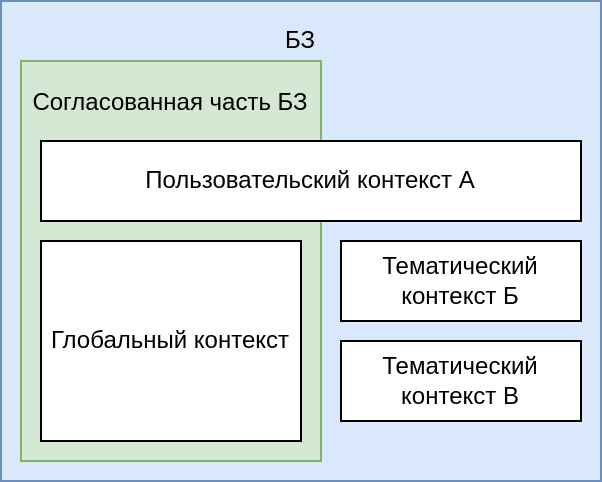
\includegraphics[scale=0.3]{images/part4/chapter_nl_interfaces/context_in_KB}
    \label{fig:context_in_KB}
\end{figure}

Подмножество \textit{контекста} может включаться в согласованную часть \textit{базы знаний}, например, если речь идет о каких-то предварительно занесенных в \textit{базу знаний} биографических сведениях --- дате рождения и тому подобном.

\begin{comment}
	

В каждый момент времени с пользователем связан 1 пользовательский диалоговый контекст (содержащий, по крайней мере известные заранее факты о нем: имя, возраст и тому подобное) и несколько тематических.
Пример спецификации контекстов представлен на~\textit{\nameref{fig:user_context}}.

\begin{figure}[H]
    \caption{SCg-текст. Иллюстрация спецификации контекстов.}
    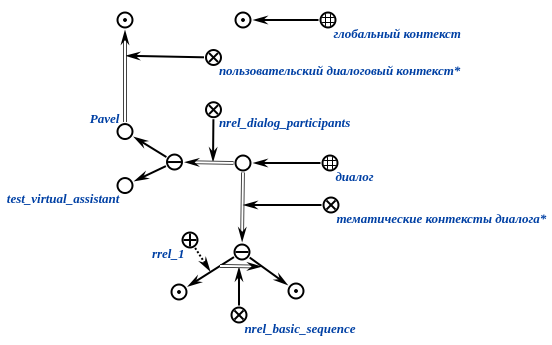
\includegraphics[scale=0.8]{images/part4/chapter_nl_interfaces/user_context}
    \label{fig:user_context}
\end{figure}

Так, \textbf{\textit{действие. разрешение контекста}} сводится к сопоставлению каждому варианту его значения соответствующего \textit{контекста}.
Выбор производится на основании значения функции \textit{$F_{CTD}(T, C)$}, где \textit{T} --- \textit{вариант трансляции}, \textit{C} --- \textit{тематический контекст}.
Подходящим контекстом для варианта трансляции считается тот, для которого значение этой функции максимально.
В случае, если подходящий контекст не найден, генерируется новый.
Пример результата данного действия представлен на~\textit{\nameref{fig:relevant_contexts}}.

\begin{figure}[H]
    \caption{SCg-текст. Иллюстрация сообщения, всем вариантам значения которого сопоставлен контекст.}
    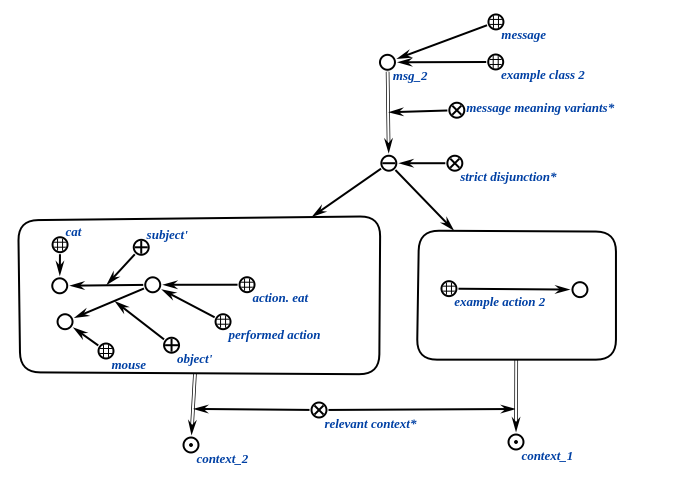
\includegraphics[scale=0.8]{images/part4/chapter_nl_interfaces/relevant_contexts}
    \label{fig:relevant_contexts}
\end{figure}

\textbf{\textit{действие. выбор смысла сообщения}} представляет собой выбор из множества вариантов трансляции и соответствующих им \textit{контекстов} одной пары и обозначение ее как эквивалентной сообщению конструкции.
В простейшем случае, на данном этапе допустимо выполнить выбор в соответствии с рассчитанными на предыдущем этапе для пар потенциально эквивалентных структур и соответствующих им \textit{контекстов} значениями функции \textit{$F_{CTD}(T, C)$} и выбрать пару, для которой оно максимально, однако при необходимости также возможно введение и отдельной функции.
Пример результата данного действия представлен на~\textit{\nameref{fig:message_equivalent_structure}}.

\begin{figure}[H]
    \caption{SCg-текст. Иллюстрация конструкции, описывающей эквивалентную сообщению структуру.}
    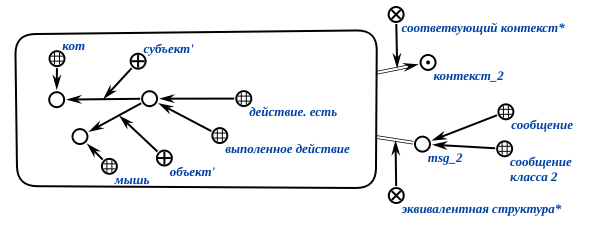
\includegraphics[scale=0.8]{images/part4/chapter_nl_interfaces/message_equivalent_structure}
    \label{fig:message_equivalent_structure}
\end{figure}

\textbf{\textit{Действие. погружение сообщения в контекст}} представляет собой погружение полученного смысла сообщения в \textit{контекст}.
Кроме выбранного смысла сообщения, в контекст может добавляться и иная необходимая для обработки сообщения информация.
Кроме того, на данном этапе на основе хранящихся в контексте сведений также должно выполняться разрешение местоимений.
Примеры \textit{контекста} до погружения в него сообщения и после погружения представлены на~\textit{\nameref{fig:context_before_update}} и~\textit{\nameref{fig:updated_context}}.

\begin{figure}[H]
    \caption{SCg-текст. Иллюстрация контекста до погружения сообщения.}
    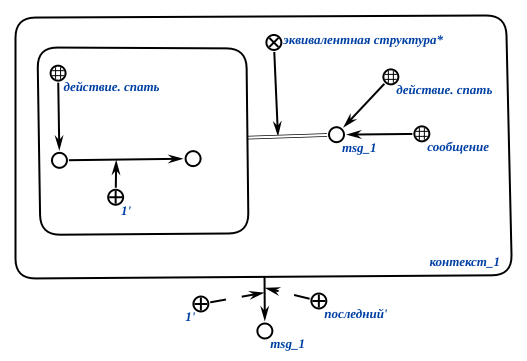
\includegraphics[scale=0.8]{images/part4/chapter_nl_interfaces/context_1}
    \label{fig:context_before_update}
\end{figure}

\begin{figure*}[h]
	\caption{SCg-текст. Иллюстрация контекста после погружения сообщения.}
    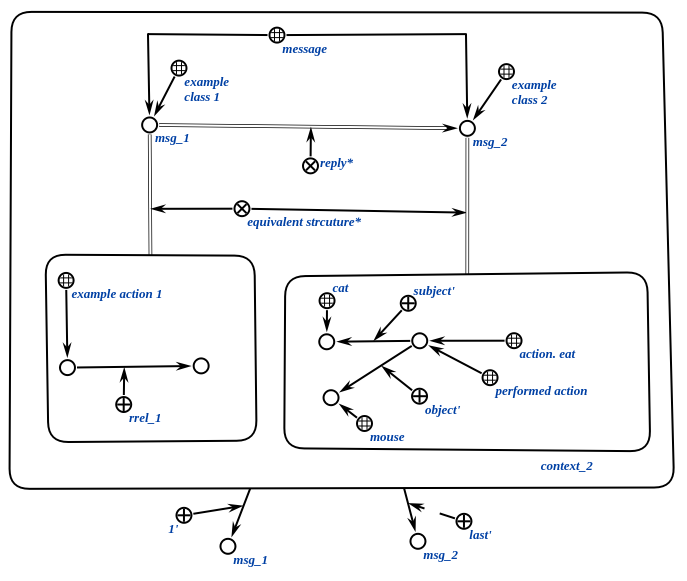
\includegraphics[scale=0.8]{images/part4/chapter_nl_interfaces/context_2}
    \label{fig:updated_context}
\end{figure*}

Таким образом, актуальная информация собирается в тематический контекст, объединив который с контекстом пользователя и глобальным контекстом можно получить общий контекст, на основании которого должны осуществляться требуемые действия системы, включая генерацию ответа системы.

\section{Методика и средства разработки естественно-языковых интерфейсов}
\label{section_natural_language_interface_development_methods}

Методика разработки естественно-языковых интерфейсов включает несколько этапов, в которых необходимо учитывать методику построения и модификации гибридных баз знаний и гибридных решателей задач (см. \scncite{Davydenko2018}, см. \scncite{Shunkevich2018}).

На~\textit{\nameref{fig:method-interface}} представлен перечень таких этапов с указанием последовательности их выполнения.

\begin{figure}[H]
	\caption{Рисунок. Этапы процесса разработки естественно-языкового интерфейса}
	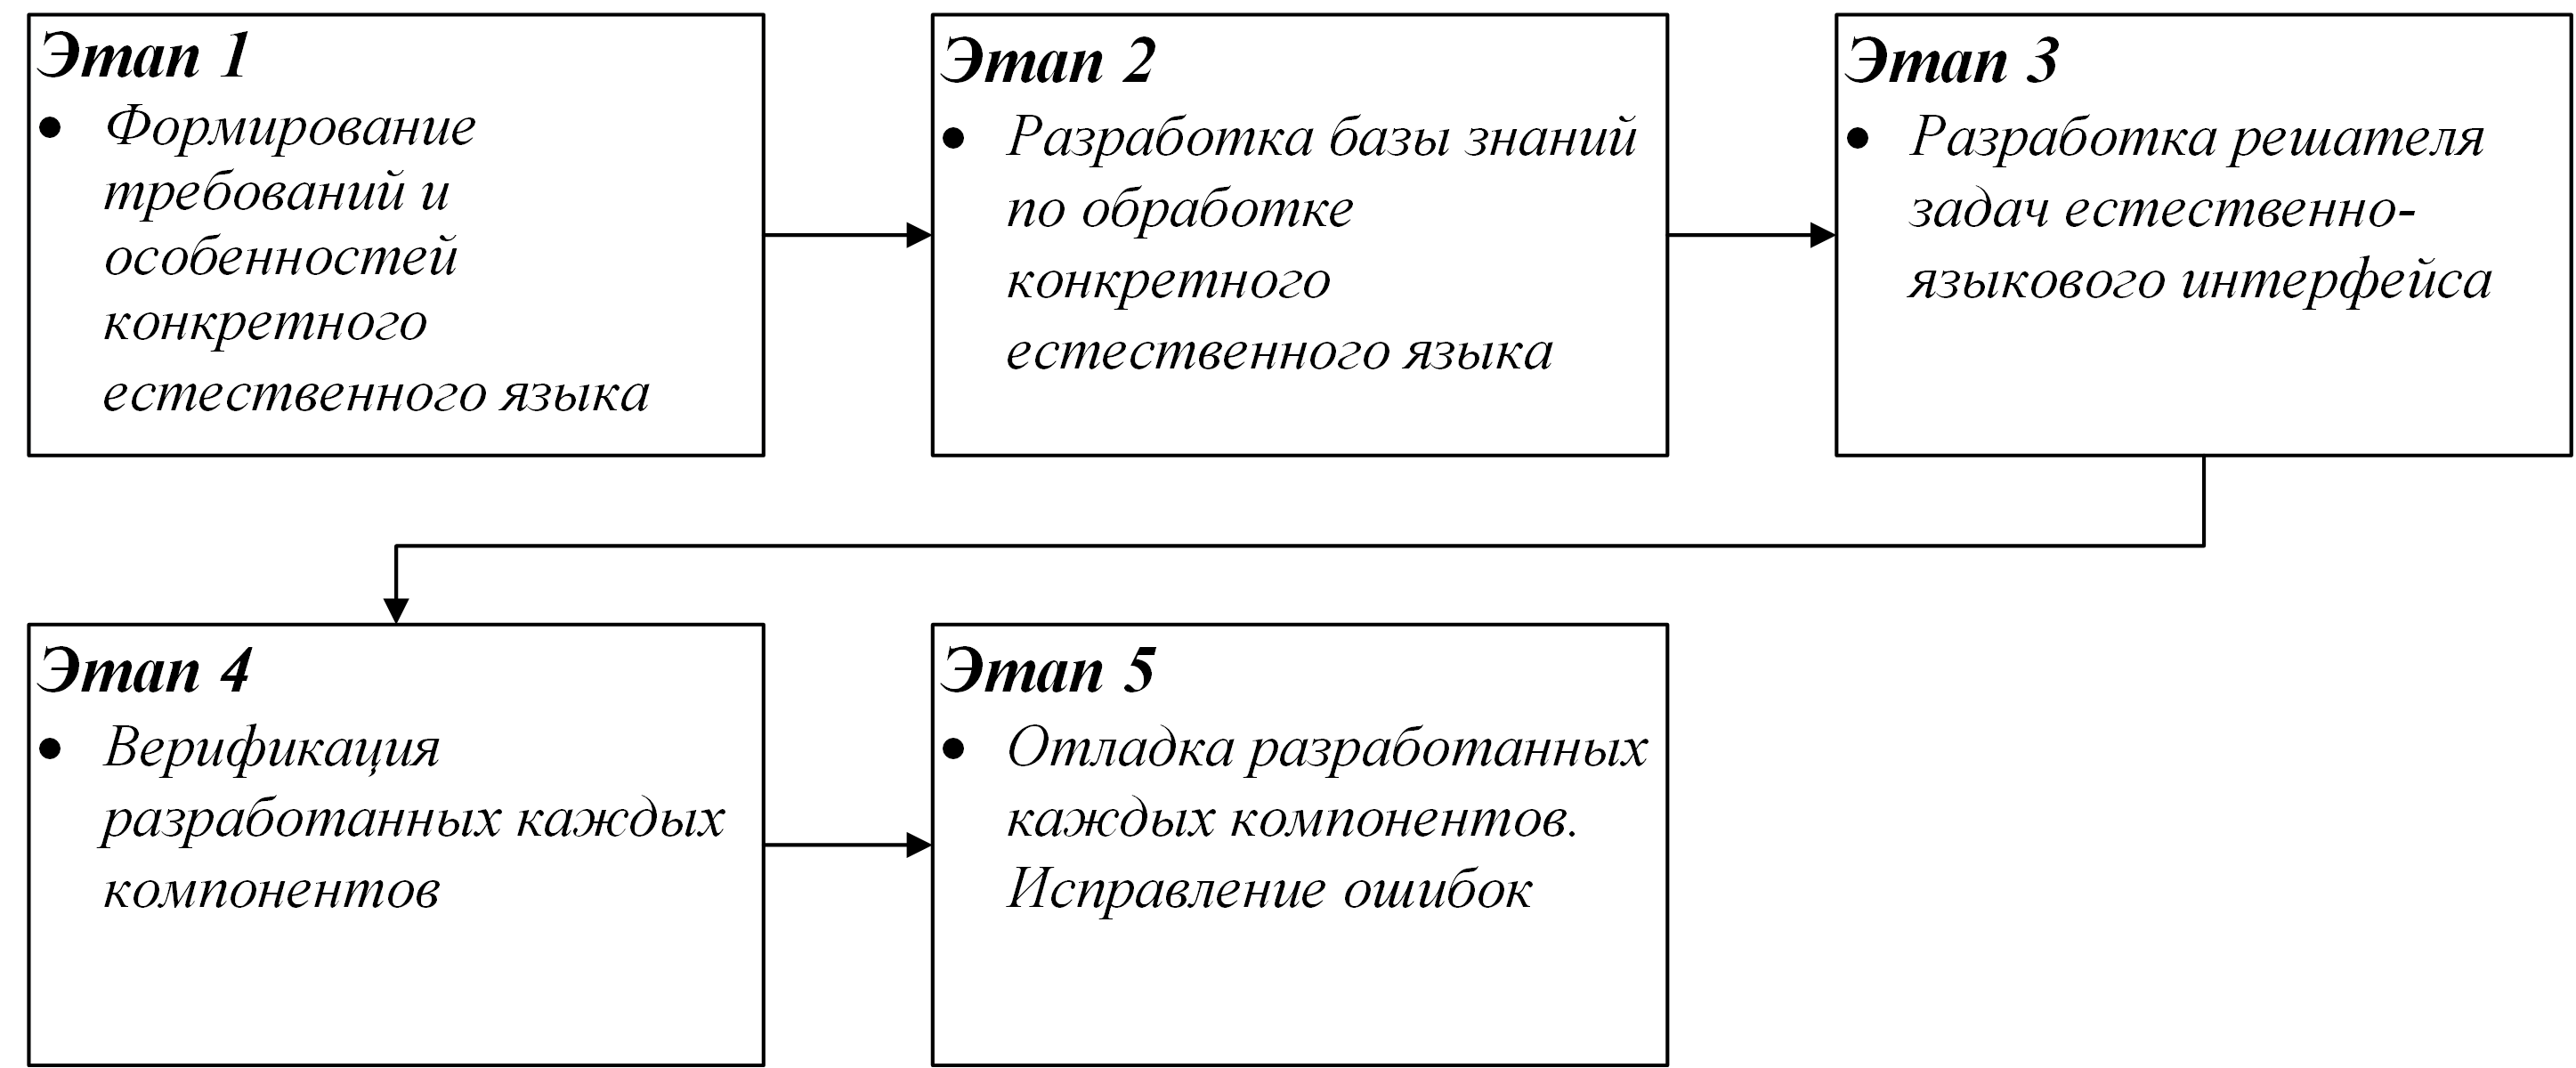
\includegraphics[scale=0.8,width=1.0\textwidth]{images/part4/chapter_chinese/method}
	\label{fig:method-interface}
\end{figure}

Данная методика может быть применена при разработке конкретного естественно-языкового интерфейса по конкретной предметной области.

Далее рассмотрим этапы процесса разработки естественно-языкового интерфейса ostis-систем:

\textbf{Этап 1. Формирование требований с учетом особенностей конкретного естественного языка.}

На данном этапе необходимо четко рассматривать особенности конкретного \textit{естественного языка}.
Затем можно разработать базу знаний по обработке конкретного \textit{естественного языка} и соответствующие \textit{решатели задач} для выполнения обработки.
После определения конкретного \textit{естественного языка} существует вероятность того, что в составе библиотеки компонентов уже есть реализованный вариант требуемой базы знаний и соответствующих решателей.
В противном случае, тем не менее, у разработчика появляется возможность включить разработанную \textit{базу знаний} по обработке конкретного естественного языка и соответствующие \textit{решатели задач} в \textit{библиотеку компонентов} для последующего использования.

\textbf{Этап 2. Разработка базы знаний по обработке конкретного естественного языка.}

На данном этапе при разработке базы знаний используются общие принципы согласованного построения и модификации \textit{гибридных баз знаний} (см. \scncite{Davydenko2017}).

\textbf{Этап 3. Разработка решателей задач естественно-языковых интерфейсов.}

Для разработки \textit{решателей задач} \textit{естественно-языкового интерфейса}, направленных на приобретение фактографических знаний и генерацию текстов конкретного \textit{естественного языка}, используются общие принципы согласованного построения и модификации гибридных \textit{решателей задач} (см. \scncite{Shunkevich2018}).

\textbf{Этап 4. Верификация разработанных компонентов.}

На данном этапе выполняется верификация разработанных \textit{компонентов} (\textit{базы знаний} по обработке конкретного естественного языка и соответствующего \textit{решателя задач}) конкретного \textit{естественно-языкового интерфейса}.

\textbf{Этап 5. Отладка разработанных компонентов. Исправление ошибок.}

Как правило, этапы 4 и 5 могут выполняться циклически до тех пор, пока разработанные компоненты не будут соответствовать предъявляемым требованиям.

\textit{Библиотека многократно используемых компонентов} является важнейшим понятием в рамках \textit{Технологии OSTIS} (см. \textit{Главу~\ref{chapter_library}~\nameref{chapter_library}}).
Библиотека многократно используемых компонентов естественно-языковых интерфейсов позволяет выбрать компоненты уже разработанные компоненты и включить их в разрабатываемый \textit{естественно-языковой интерфейс} других \textit{ostis-систем}, то есть разработанные компоненты \textit{естественно-языковых интерфейсов} могут быть повторно использованы при разработке естественно-языковых интерфейсов в других \textit{ostis-системах}.
Ниже предложена структура библиотеки многократно используемых компонентов \textit{естественно-языковых интерфейсов}.
\begin{SCn}
	\scnheader{Библиотека многократно используемых компонентов естественно-языковых интерфейсов}
	\begin{scnrelfromset}{разбиение}
		\scnitem{Библиотека многократно используемых компонентов базы знаний естественно-языковых интерфейсов}
		\begin{scnindent}
			\scnidtf{Библиотека многократно используемых компонентов лингвистической базы знаний}
			\scnidtf{Библиотека многократно используемых компонентов базы знаний по обработке естественного языка}
		\end{scnindent}
		\scnitem{Библиотека многократно используемых компонентов решателей задач естественно-языковых интерфейсов}
		\begin{scnindent}
			\scnidtf{Библиотека многократно используемых компонентов решателей задач для обработки естественного языка}
		\end{scnindent}
	\end{scnrelfromset}
\end{SCn}

При необходимости, \textit{библиотеку многократно используемых компонентов} \textit{естественно-языковых интерфейсов} можно дополнять знаниями о конкретных \textit{естественных языках}.
Ниже представлен пример структуры библиотеки многократно используемых компонентов для построения китайско-языкового интерфейса.

\begin{SCn}
	\scnheader{Библиотека многократно используемых компонентов китайско-языкового интерфейса}
	\begin{scnrelfromset}{разбиение}
		\scnitem{Библиотека многократно используемых компонентов базы знаний китайско-языкового интерфейса}
		\begin{scnindent}
			\scnidtf{Библиотека многократно используемых компонентов базы знаний по обработке китайского языка}
		\end{scnindent}
		\scnitem{Библиотека многократно используемых компонентов решателей задач китайско-языкового интерфейса}
		\begin{scnindent}
			\scnidtf{Библиотека многократно используемых компонентов решателей задач для обработки китайского языка}
		\end{scnindent}
	\end{scnrelfromset}
\end{SCn}
\end{comment}